\documentclass[twoside, letterpaper, 12pt]{report}
\usepackage{orthodoxservicebook}

\title{The Sunday Reader's Service of the \\ \textsc{Typica} \\ 2020 April 05}
\titlepic{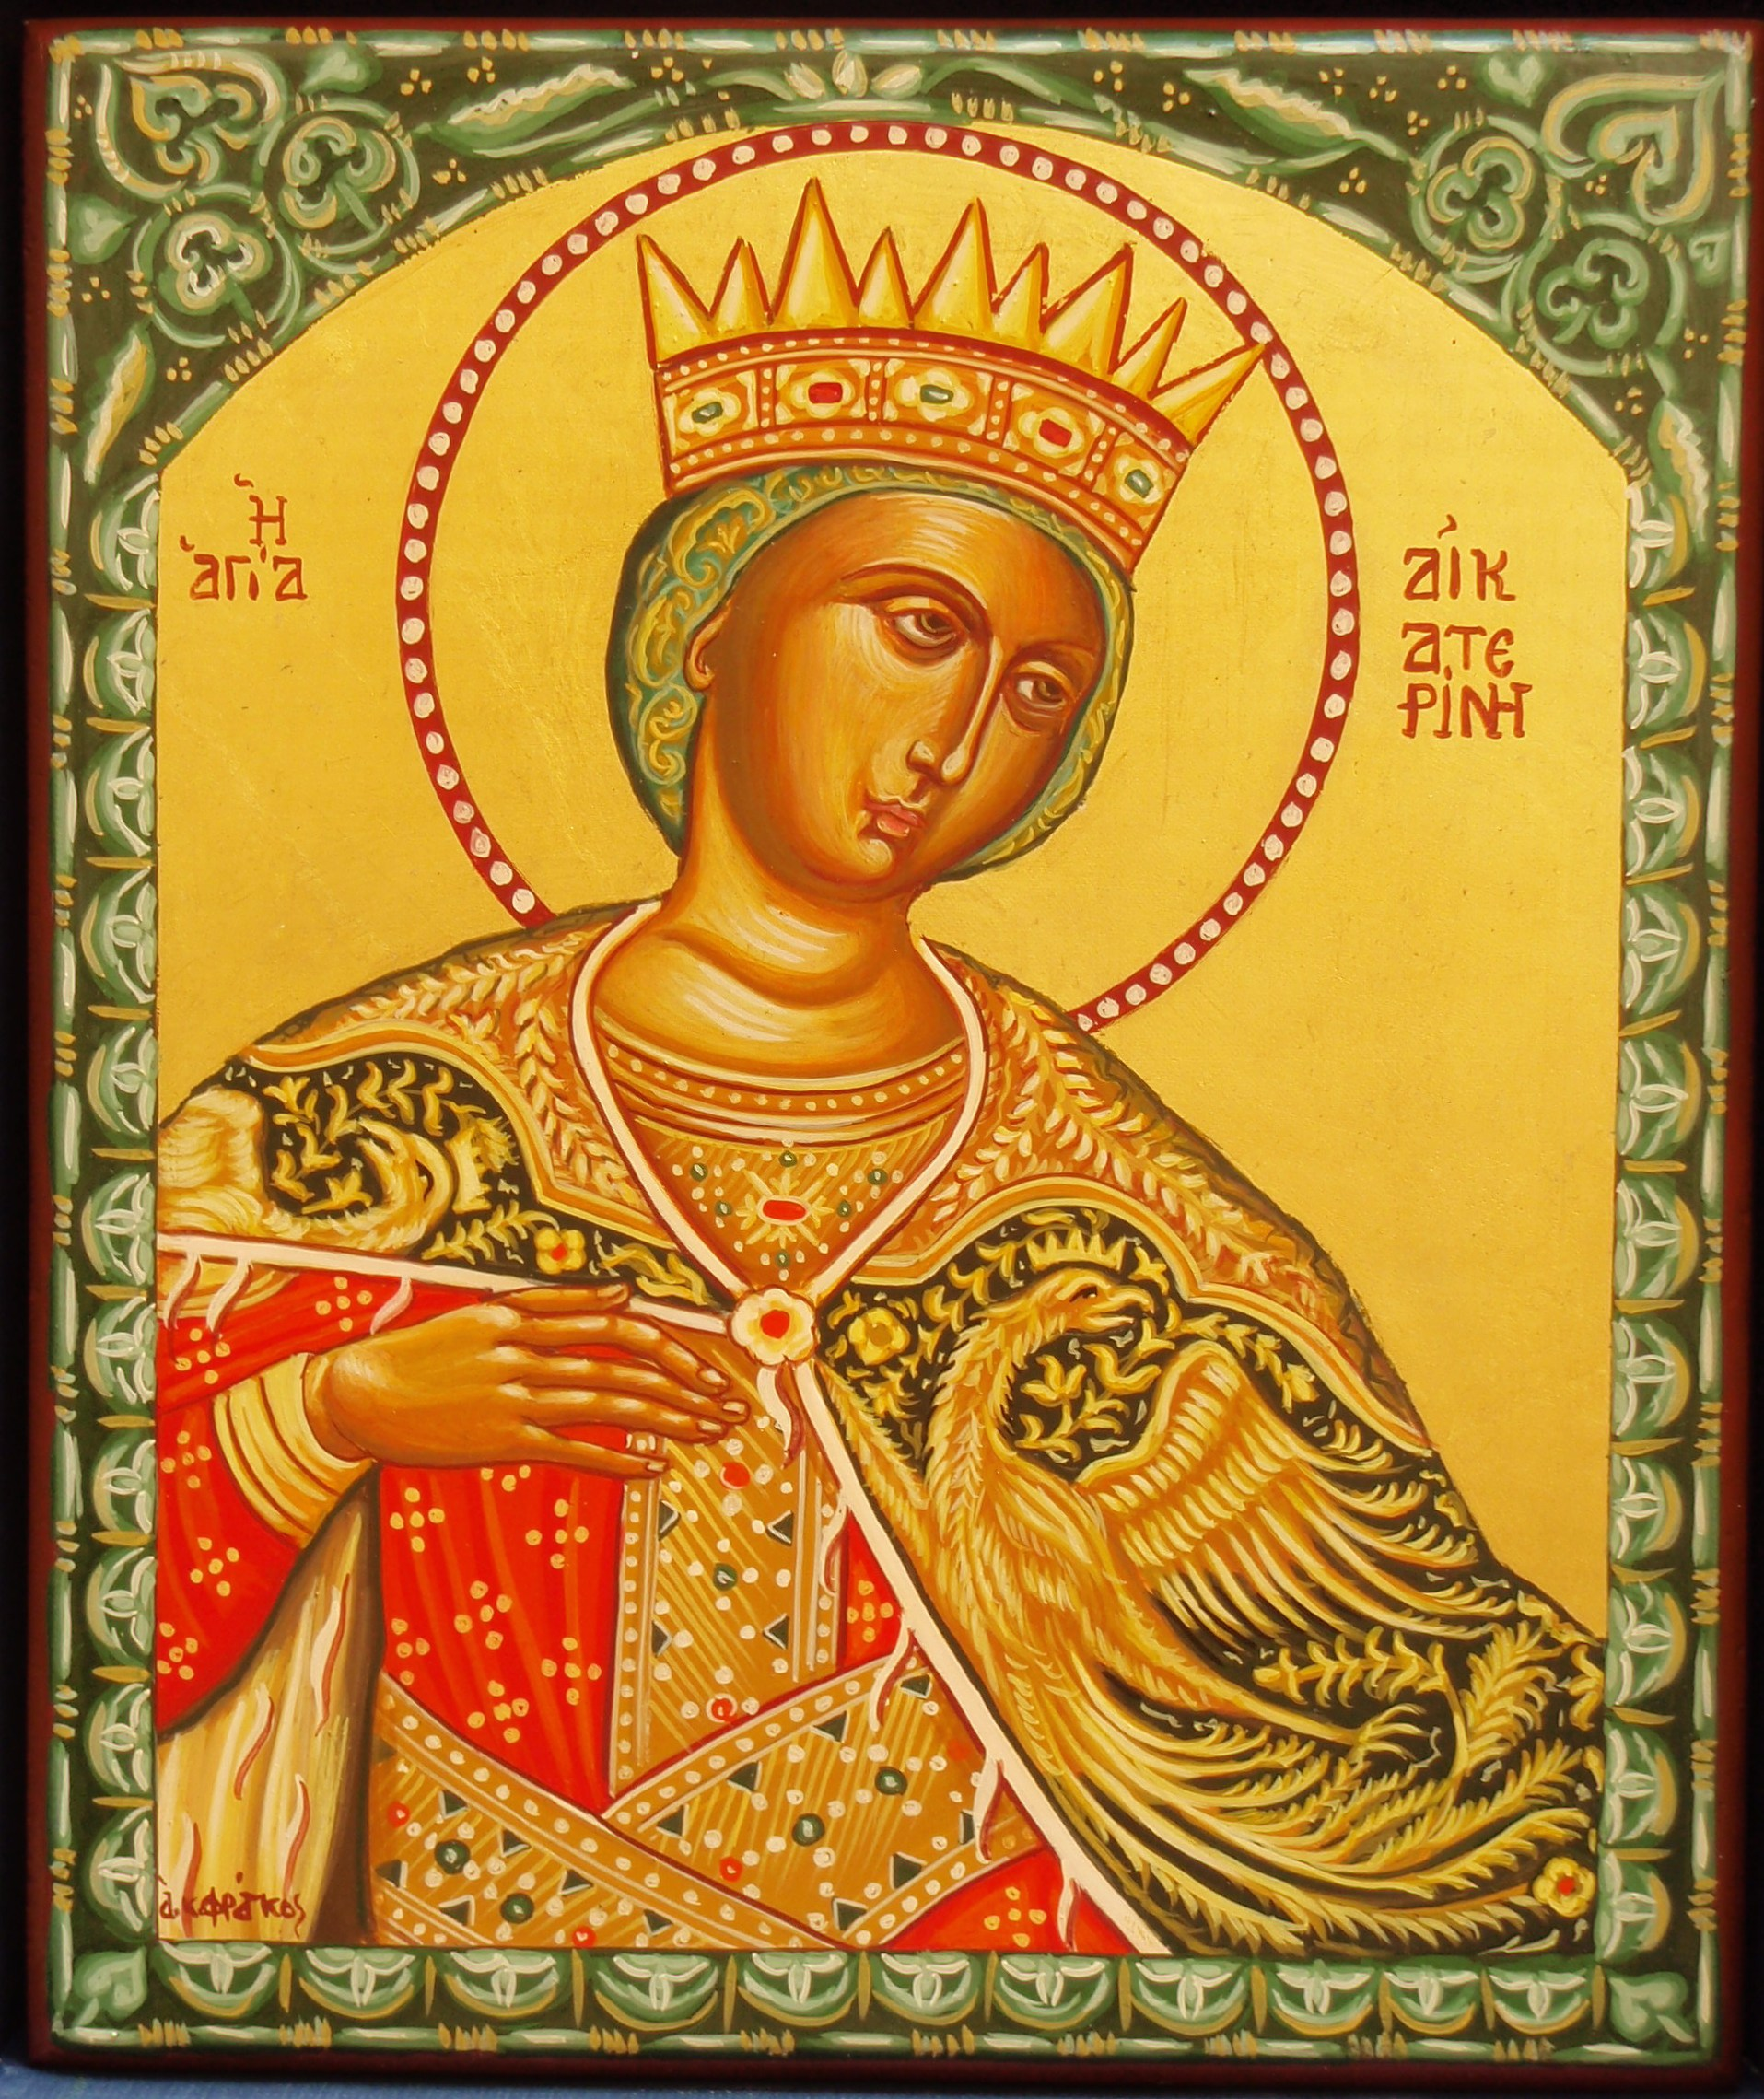
\includegraphics[width=0.5\textwidth]{Katherine1.jpg}}
\date{}
\author{}

\begin{document}
\maketitle
\pagestyle{empty} % Don't show page numbers
\instruction{This page intentionally left blank}
\cleardoublepage
\pagestyle{plain}
\setcounter{page}{1} % Set the page counter to 1 on the first real page
\chapter*{The Sunday Reader's Service of Typica\\ 2020 April 05}
\readerline{Through the prayers of our holy fathers, Lord Jesus Christ our God,
  have mercy on us, and save us}
\lilypondfile{./Z-Responses/Obikhod/Amen.ly}

\trisagionNeedsAmen[reader]
\lilypondfile{./Z-Responses/Obikhod/Amen.ly}


\centeredsection{The First Antiphon}
\lilypondfile{./Liturgy/B-FirstAntiphon/BlessTheLord_Greek-Music.ly}

\centeredsection{The Second Antiphon}
\lilypondfile{./Liturgy/C-SecondAntiphon/PraiseTheLord_Greek-Music.ly}

\centeredsection{The Third Antiphon}
\lilypondfile{./Liturgy/D-ThirdAntiphon/Beatitudes_Moscow-Music.ly}

\centeredsection{The Epistle}

\instruction{Both of the New Testament lessons are read
without liturgical introduction or conclusion.
The readers start with “The Reading from…” and proceeds}

\paragraph{The Reading from the Epistle of St. Paul to the Hebrews. (9:11-14)}\mbox{}\\

Brethren, when Christ appeared as a high priest of the good things that have come,
then through the greater and more perfect tent
(not made with hands, that is, not of this creation),
He entered once for all into the Holy Place,
taking not the blood of goats and calves but His own blood,
thus securing an eternal redemption.
For if the sprinkling of defiled persons with the blood of goats and bulls and with the ashes of a
heifer sanctifies for the purification of the flesh, how much more shall the blood of Christ,
Who through the eternal Spirit offered Himself without blemish to God,
purify your conscience from dead works to serve the living God?

\centeredsection{The Gospel}

\instruction{Both of the New Testament lessons are read
without liturgical introduction or conclusion.
The readers start with “The Reading from…” and proceeds}

\paragraph{The Reading from the Holy Gospel according to St. Mark. (10:32-45)}\mbox{}\\

At that time, Jesus took His twelve Disciples, and began to tell them what was to happen to Him,
saying, “Behold, we are going up to Jerusalem.
And the Son of man will be delivered to the chief priests and the scribes,
and they will condemn Him to death, and deliver Him to the Gentiles.
And they will mock Him, and scourge Him, and spit upon Him, and kill Him;
and after three days He will rise.”
And James and John, the sons of Zebedee, came forward to Him, and said to Him,
“Teacher, we would that thou shouldest do for us whatsoever we shall desire.”
And Jesus said to them, “What do you want Me to do for you?” And they said to Him,
“Grant us to sit, one at Thy right hand and one at Thy left, in Thy glory.”
But Jesus said to them, “You do not know what you are asking.
Are you able to drink the cup thatI drink,
or to be baptized with the baptism with which I am baptized?”
And they said to Him, “We are able.”
And Jesus said to them, “The cup that I drink you will drink;
and with the baptism with which I am baptized, you will be baptized.
But to sit at My right hand or at My left is not Mine to grant,
but it is for those for whom it has been prepared.”
And when the ten heard it, they began to be indignant at James and John.
And Jesus called them to Him and said to them,
“You know that those who are supposed to rule over the Gentiles lord it over them,
and their great men exercise authority over them.
But it shall not be so among you; But whoever would be great among you must be your servant,
and whoever would be first among you must be servant of all.
For the Son of man also came not to be served but to serve,
and to give His life as a ransom for many.”

\centeredsection{Troparia Before the Creed}
\instruction{Plain reading}
\begin{reader}
\item[Reader 1:] The heavenly choir singeth thy praises, saying:
  Holy, holy, holy, Lord of Sabaoth; heaven and earth are full of Thy glory.

\item[Reader 2:] \emph{Come unto him, and be enlightened,
               and your faces shall not be ashamed.}
  The heavenly choir singeth thy praises, saying:
  Holy, holy, holy, Lord of Sabaoth; heaven and earth are full of Thy glory.

\item[Reader 1:] \emph{\glory}
  The choir of the holy angels and archangels,
  with all the powers of heaven, singeth thy praises, saying:
  Holy, holy, holy, Lord of Sabaoth; heaven and earth are full of Thy glory.

\item[Reader 2:]\emph{\nowandever}
\end{reader}

\centeredsection{The Creed}
\input{Common/TheCreed.txt}


\centeredsection{Prayer of Forgiveness}
\readerline{Forgive, remit, pardon, O God, our sins,
  both voluntary and involuntary, in deed and in word, in knowledge or in ignorance,
  committed by night or by day, in mind and in thought.
  Forgive us them all, for thou art good and lovest mankind.
}


\centeredsection{The Lord’s Prayer}
\input{Common/LordsPrayer.txt}

\readerline{Through the prayers of our holy fathers, Lord Jesus Christ our God, have mercy on us.}
\lilypondfile{./Z-Responses/Obikhod/Amen.ly}


\centeredsection{Kontakia for normal Sundays}
\lilypondfile{./Liturgy/H-Kontakion/OProtectionOfChristians_Tone2ByzChant-Music.ly}


\readerline{\lhmForty}

\readerline{
  O Christ our God, Who art worshipped and glorified at all times at every hour both in
  heaven and on earth; Who art long-suffering and plenteous in mercy and compassion; Who lovest
  the just man and showest mercy upon the sinner; and Who callest all men to repentance through 
  the promise of blessings to come; receive, O Lord, at this very hour our supplications, and direct
  our lives in the way of Thy commandments: sanctify our souls, purify our bodies, set our minds
  aright, cleanse our thoughts; deliver us from all affliction, trouble, and distress; compass us about
  with Thy holy angels, that, guided and guarded by them, we may attain unto the unity of the Faith,
  and to the knowledge of Thine unapproachable glory; for Thou art blessed unto ages of ages. Amen.
}

\begin{reader}
  \item \lhmThree{}\\\emph{\gne{}}
  \item \morehonorablethanthetherubim{}
  \item \throughtheprayers{}
\end{reader}

\begin{maybetwocolumns}
\lilypondfile{./Z-Responses/Obikhod/Amen.ly}

\readerline{\blessedbethename{}\thrice{}}

\centeredsection{Psalm 33}
\input{./Psalms/Psalm033-unknowntrans.txt}

\centeredsection{Psalm 144}
\input{./Psalms/Psalm144-unknowntrans.txt}
\end{maybetwocolumns}

\peopleline{\gne}


\centeredsection{A Homily}
\begin{maybetwocolumns}
\instruction{5th Sunday of lent, third Sunday of Quarantine
Selfless Service Over Self-Centered Desire:
Homily for the FifthSunday of Lent in the Orthodox Church
Fr. Philip LeMasters, pastor, St. Luke Antiochian Orthodox Church of Abilene, Texas}

Human beings have an amazing capacity to miss the point,
to become blind to truths that should be obvious. 
We often do that because we become so preoccupied and distracted with our own agendas
and desires that we ignore everything else.
That is especially the case when the truth goes strongly against our inclinations by
telling us what we do not want to hear.

That is what James and John did when they asked for choice positions of honor right after
Jesus Christ had told them that He was to suffer, die, and rise from the dead.
They were apparently so consumed by their desires for prominence and power that they
refused to hear the Lord saying that He was nothing like an earthly king.
They boasted of being prepared to follow the Savior without having any idea of what that
would mean.
He responded by making clear that the path to true greatness was to follow His way of
selfless service. “For the Son of man also came not to be served but to serve,
and to give His life as a ransom for many.

”As we begin the last week of Lent,
it should be clear to us all that we have not earned a place of honor in God’s reign.
If we have practiced the spiritual disciplines of Lent with any integrity and honesty,
we will know primarily our own weakness and brokenness.
By revealing how easily we are distracted and how enslaved we are to our
self-centered desires and habits, they show us that we cannot heal our own souls.
And if we have not devoted ourselves to prayer, fasting, 
and almsgiving at all in the previous weeks of Lent,
we should confess that in humility and thus gain a greater awareness that we stand in
constant need of the Lord’s gracious mercy.
“Lord Jesus Christ, Son of God, have mercy on me, a sinner.

”Regardless of how we have approachedLent so far,
we must not become paralyzed with a sense of obsessive guilt for not living up to a
standard of perfection, for not making ourselves worthy of the mercy of Christ.
To do so is simply a form of self-centered pride,
for it is impossible to earn grace as a reward for good behavior.
Becoming great among the Lord’s servants means laying down our lives for others,
lowering ourselves by placing the needs and interests of others before our own.
That is the opposite of a self-centered obsession to prove that we are worthy of anything.

Today we remember St. Mary of Egypt, who had lived a grossly immoral life,
but then gave herself up in repentance for decades in the desert,
where she became a remarkably holy saint. Instead of continuing to gratify her addiction
to sexual pleasure, she died to self by rejecting everything that was a hindrance to the
healing of her soul through incredibly rigorous repentance for the rest of her long life.
She knew that such disciplines did not somehow put God in her debt,
but were ways of opening herself to receive the gracious healing of the Lord,
which we never deserve.

St. Mary of Egypt was not like James and John in trying to use the Savior to get what she wanted.
Instead, she freely obeyed a divine command to turn away from fulfilling her obsessive desires by
uniting herself to the One Who offered His life as a ransom to free us all from slavery to sin
and death. Our Lord’s disciples ultimately found victory over their passions in different ways,
for they had to learn that greatness in the Kingdom comes through selfless service to the point of
suffering and death, not by yearning after what the world calls power and success.

In the remaining days of Lent, we all have the opportunity to embrace our Lord’s way of selfless
service in relation to those we encounter on a regular basis in our families, in our parish,
at work, at school, and in our larger communities.
We all have the opportunity to confess how we have enslaved ourselves to self-centered desires
and then to take the steps we can to turn away from them. 
We all have the opportunity to fill our minds with holy things and give less attention to whatever
fuels our unholy passions.
We all have the opportunity to follow the example of St. Mary of Egypt in doing what it takes to
find the healing of our souls. If our Lord could make a great saint out of her,
then how can anyone remain paralyzed in guilt? Our great High Priest offered Himself on the Cross
and rose in glory on the third day in order to save sinners,
to restore all who bear His image and likeness.
Thanks be to God, that includes even people as broken as you and me.
In the coming week, let us open the eyes of our souls to this glorious truth through selfless
service, humble prayer, and genuine repentance.

\end{maybetwocolumns}

\centeredsection{Resurrectional Apolytikion in Tone 1}
\lilypondfile{./Octoechos/ResurrectionalApolytikion-Tone1-Kazan-Music.ly}

\centeredsection{Apolytikion of St. Mary of Egypt in Tone 8}

Through thee, the divine likeness was securely preserved, O mother Mary;
for thou didst carry the cross and follow Christ.
By example and precept thou didst teach us to ignore the body, because it is perishable,
and to attend to the concerns of the undying soul.
Therefore, doth thy soul rejoice with the angels.

\readerline{\throughtheprayers}

\lilypondfile{./Z-Responses/Obikhod/Amen.ly}

\end{document}

